\paragraph{Sort-Merge Join}
Example:
\begin{lstlisting}
  SELECT *
  FROM Reserves R1, Sailors S1
  WHERE R1.sid=S1.sid
\end{lstlisting}

\begin{enumerate}
\item Sort R on join attr(s)
\item Sort S on join attr(s)
\item Scan sorted-R and sorted-S in tandem, to find matches
\end{enumerate}

\paragraph{Cost of Sort-Merge Join}

\begin{itemize}
\item Cost: Sort R + Sort S + (|R| + |S|)
  \begin{itemize}
  \item But in the worst case, last term could be |R| $\cdot$ |S|
    (\textit{very unlikely: same values for joining
    attributes on both relations})
  \end{itemize}
\end{itemize}


Now we consider two examples which show that sort-merge join
does note improve if we already have enough memory for sorting
in 2 passes, but instead the block-nested loop can use
the additional memory

\begin{itemize}
\item Suppose B = 35 buffer pages (|R| = 1000, |S| = 500):
  \begin{itemize}
  \item both R and S can be sorted in 2 passes
  \item Total join cost = 4 $\cdot$ 1000 + 4 $\cdot$ 500
    + (1000 + 500) = 7500
  \end{itemize}
\end{itemize}

\begin{itemize}
\item Suppose B = 300 buffer pages (|R| = 1000, |S| = 500):
  \begin{itemize}
  \item Again, both R and S sorted in 2 passes
  \item Total join cost = 7500
  \end{itemize}
\end{itemize}

Using Block-Nested-Loop we would get 15000 for B = 35 and
2200 for B = 300.



An important refinement:
\begin{itemize}
\item Do the join during the final merging pass of sort!
\item If we have enough memory, can do:
  \begin{enumerate}
  \item Read R and write out sorted runs (2 |R|)
  \item Read S and write out sorted runs (2 |S|)
  \item Merge R-runs and S-runs, and find R joined S matches
    (|R| + |S|)
  \end{enumerate}

⇒ Cost = 3 $\cdot$ |R| + 3 $\cdot$ |S|
\end{itemize}

The memory requirement: B > $\sqrt{|\text{R}| + |\text{S}|}$

Sort-merge join an especially good choice if:
\begin{itemize}
\item one or both inputs are already sorted on join attribute(s)
\item output is required to be sorted on join attribute(s)
\end{itemize}


\paragraph{GRACE Hash Join}
\begin{itemize}
\item partition both relations using hash function h:
  R tuples in partition $i$ will only match S tuples in
  partition $i$
\item R join S = $\text{R}_1$ join $\text{S}_1 \cup \text{R}_2$
  join $\text{S}_2 \cup \cdots \cup \text{R}_{\text{B}-1}$ join
  $\text{S}_{\text{B}-1}$
\end{itemize}

\begin{itemize}
\item Partitioning phase:
  read + write both relations
  ⇒ 2(|R| + |S|) I/Os

\item Matching phase:
  read both relations
  ⇒ |R| + |S| I/Os

\item If memory is enough (assuming R smaller than B > $\sqrt{R}$ is
  enough memory),
  2-pass hash join cost = 3(|R| + |S|)
\end{itemize}

\paragraph{2-Pass Hash Join vs. 2-Pass Sort-Merge Join}
\begin{itemize}
\item Given ``enough'' memory, both have cost of
  3 (M + N)

\item Benefits of hash join
  \begin{itemize}
  \item Superior if relation sizes differ greatly
  \item \textbf{Refinement:} hybrid hash join allows for dynamically
    adjusting to smaller relation fitting in main memory
  \item Highly parallelizable
  \end{itemize}

\item Benefits of sort-merge join
  \begin{itemize}
  \item Less sensitive to data skew
  \item Result is sorted
  \end{itemize}
\end{itemize}


\paragraph{Set Operations}
\begin{itemize}
\item Intersection and cross-product special cases of join
\item Union (Distinct) and Except are similar; we discuss union
\end{itemize}

\begin{itemize}
\item \textbf{Sorting based approach to union:}
  \begin{itemize}
  \item Sort both relations (on combination of all attributes)
  \item Scan sorted relations and merge them
  \item Alternative: Merge runs from Pass 0 for both relations
  \end{itemize}

\item \textbf{Hash based approach to union:}
  \begin{itemize}
  \item Partition R and S using hash function h
  \item For each S-partition, build in-memory hash table
    (using h2), scan corresponding R-partition and add
    tuples to output while discarding duplicates
  \end{itemize}
\end{itemize}

\paragraph{Query Execution Framework}
Example:
\begin{lstlisting}
  SELECT DISTINCT name, gpa
  FROM Students
\end{lstlisting}

One possible \textbf{query execution plan:}

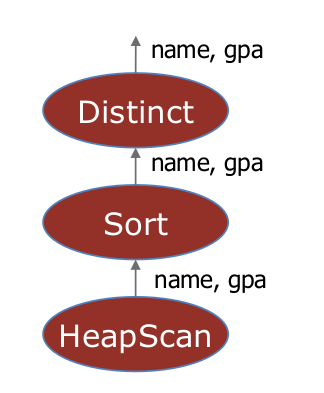
\includegraphics[scale=0.15]{graphics/qu-ex-plan.png}


\paragraph{Design Goals for Operator Interface}
\begin{itemize}
\item Must be able to compose several operators together into
  operator tree
\item Must coordinate how data is passed between operators
\item Should only buffer necessary data in main memory
\end{itemize}


\paragraph{Pull Model}
\begin{itemize}
\item User requests one tuple at a time from top-level operator
\item Operators calculate next tuple by requesting tuples from their
  input operators
\end{itemize}

ONC-Interface (iterator)
\begin{itemize}
\item \textbf{Open:} initializes the operator
\item \textbf{Next:} Calculates the next tuple and returns it to caller
\item \textbf{Close:} Cleans up and closes operator
\end{itemize}


\section{Parallel Data Processing}

\paragraph{Why Parallel Access to Data?}
\begin{itemize}
\item \textbf{Take 1 TB of data}
  \begin{itemize}
  \item at 10 MB/s → 1.2 days to scan
  \item 1000x parallel → 1.5 minute to scan
  \end{itemize}
\item \textbf{Bandwidth!}
\item \textbf{Parallelism}
  \begin{itemize}
  \item Divide big problem into many smaller ones to be
    solved in parallel
  \item Take advantage of natural independence among
    portions of processing
  \end{itemize}
\end{itemize}


\paragraph{Parallel Databases: Intro}

\begin{itemize}
\item Parallelism is natural to data processing
  \begin{itemize}
  \item \textit{Pipeline parallelism:} many machines each doing
    one step in a multi-step process
  \item \textit{Partition parallelism:} many machines doing the
    same thing to different pieces of data
  \item \textbf{Both are natural in database systems!}
  \end{itemize}
\end{itemize}


Database systems are the most successful application of parallelism

Reasons for success:
\begin{itemize}
\item \textbf{A close set of operators with well-defined semantics}
  \begin{itemize}
  \item Fully optimized implementations
  \item Automatic optimizer
  \end{itemize}

\item \textbf{Bulk-processing} (= partition parallelism):
  Natural pipelining
\item \textbf{Inexpensive hardware} can do the trick!
\item Users/app-programmers
  \textbf{do not need to think in parallelism}
\end{itemize}


\paragraph{Parallelism Terminology}

\begin{itemize}
\item Speed-Up
  \begin{itemize}
  \item More resources means proportionally less time for
    processing a given amount of data
  \end{itemize}

\item Scale-Up
  \begin{itemize}
  \item If resources increased in proportion to
    increase in data size, time is constant
  \end{itemize}
\end{itemize}


\paragraph{Architectural Issue: Shared What?}

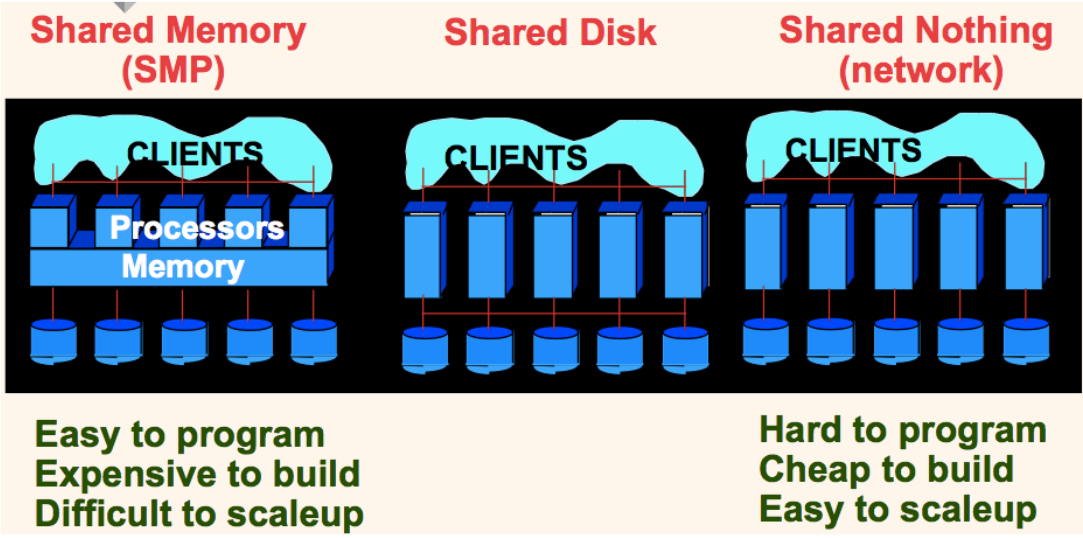
\includegraphics[scale=0.2]{graphics/shared-what.png}

\paragraph{Different Types of Database System Parallelism}
\begin{itemize}
\item Intra-operator parallelism
  \begin{itemize}
  \item get all machines working to compute a given operation
    (scan, sort, join)
  \end{itemize}

\item Inter-operator parallelism
  \begin{itemize}
  \item each operator may run concurrently on a different site
    (exploits pipelining)
  \end{itemize}

\item Inter-query parallelism
  \begin{itemize}
  \item different queries run on different sites
  \end{itemize}
\end{itemize}


\paragraph{Discussion: Automatic Data Partitioning}
\begin{itemize}
\item Round Robin
\begin{itemize}
\item generates partitions that are quite balanced, because
  the partition is not based on semantics of the data
\end{itemize}

  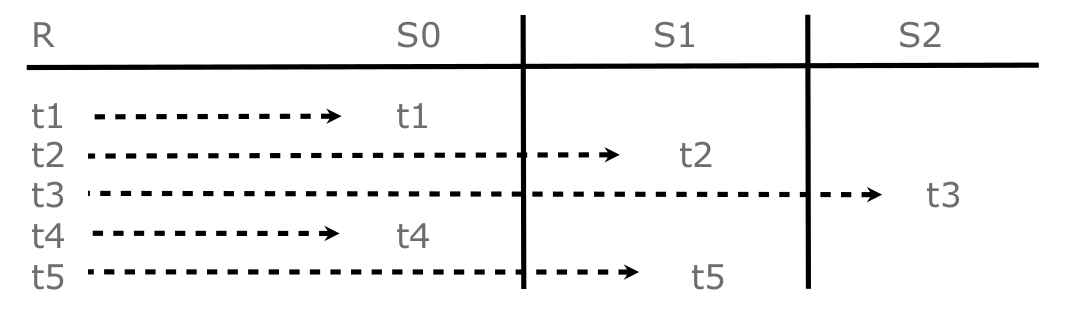
\includegraphics[scale=0.15]{graphics/round-robin.png}

\item Hash Partitioning
\begin{itemize}
\item often suffers from skewness depending on data value
\item good for hash-based algorithm
\end{itemize}


  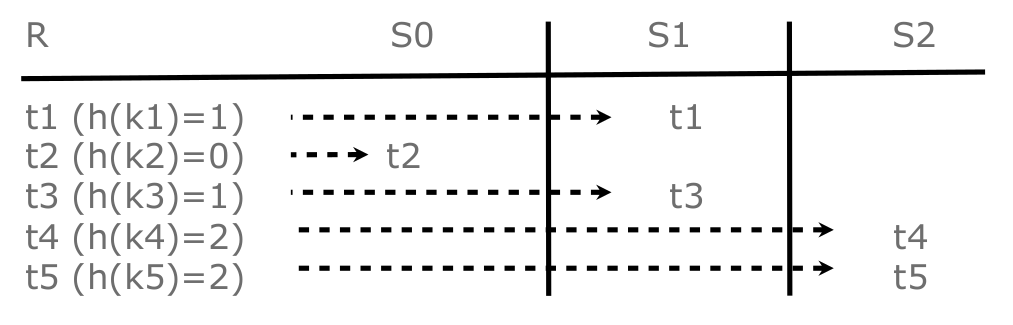
\includegraphics[scale=0.15]{graphics/hash-partitioning.png}

\item Range Partitioning
\begin{itemize}
\item can have skewness, depends how you choose range
\item good for sorting, because we can sort two partitions independently
\end{itemize}

  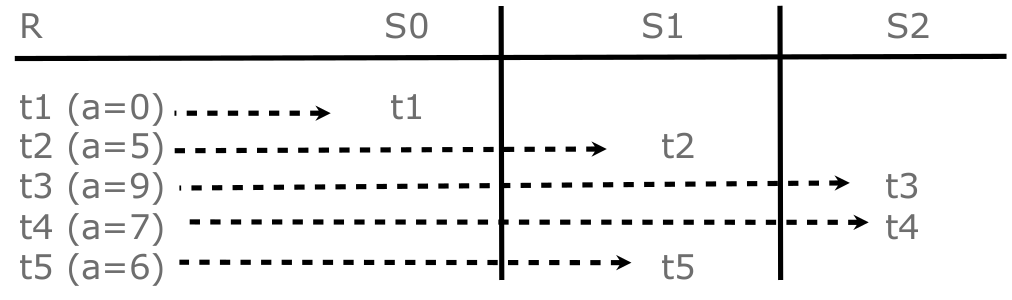
\includegraphics[scale=0.15]{graphics/range-partitioning.png}
\end{itemize}


\paragraph{Handling Skew}
\begin{itemize}
\item For range partitioning, sample load on disks
  \begin{itemize}
  \item Cool hot disks by making range smaller
  \end{itemize}

\item For hash partitioning
  \begin{itemize}
  \item Cool hot disks by making more buckets than \#nodes,
    and then mapping some buckets on hot disks to others
  \end{itemize}

\item During query processing
  \begin{itemize}
  \item Use hashing and assume uniform
  \item If range partitioning, sample data and use histogram to
    level the bulk
  \item SMP/River scheme: work queue used to balance load
  \end{itemize}
\end{itemize}


\paragraph{Parallelizing Sort}
\begin{itemize}
\item \textbf{Why?}
  \begin{itemize}
  \item DISTINCT, GROUP BY, ORDER BY, sort-merge join, index build
  \end{itemize}

\item \textbf{Phases:}
  \begin{enumerate}
  \item Redistribute data to all nodes by range partitioning
  \item Sort data in parallel
  \item Read the entire sorted relation by visiting the nodes
    in order
  \end{enumerate}

\item \textbf{Notes:}
  \begin{itemize}
  \item phase 1 requires repartitioning 1-1/n of the data! Therefore,
    High bandwidth network required
  \item phase 2\&3 totally local processing
  \item \textit{linear} speedup, scaleup
  \end{itemize}
\end{itemize}


\paragraph{Parallel Joins}
\begin{itemize}
\item Nested loop:
  \begin{itemize}
  \item Each outer tuple must be compared with each inner tuple that
    might join
  \item Easy for hash/range partitioning on join cols or
    replicating the inner table, hard otherwise!
  \end{itemize}

\item Sort-Merge (or plain Merge-Join):
  \begin{itemize}
  \item Sorting produce range-partitioned data
    \begin{itemize}
    \item R and S should use the same partitioning function
    \item skews of two relations
      \begin{itemize}
      \item Goal: $|\text{R}_i| + |\text{S}_i|$ are the same for all $i$
      \end{itemize}
    \end{itemize}
  \item Local merging of the partitioned tables
  \end{itemize}
\end{itemize}

\paragraph{Parallelizing Hash Join?}
\begin{itemize}
\item Partition both relations using hash function $h$:
  R tuples in partition $i$ will only match S tuples in
  partition $i$
\item Read in a partition of R, hash it using h2, scan
  matching partition of S, search for matches
\end{itemize}


\paragraph{Parallel Hash Join}
\begin{itemize}
\item In Phase 1, partitions get distributed to different sites:
  \begin{itemize}
  \item a good hash function automatically distributes work evenly!
  \end{itemize}

\item Do second phase at each site
\item Almost always the winner for equi-join
\end{itemize}

\paragraph{Complex Parallel Query Plans}

\begin{itemize}
\item Complex Queries: Inter-Operator parallelism
  \begin{itemize}
  \item Pipelining between operators:
    \begin{itemize}
    \item note that sort and phase 1 of hash-join block the pipeline!
    \end{itemize}
  \end{itemize}
\end{itemize}

% LocalWords:  attr parallelizable gpa ONC pipelining Intra SMP equi
% LocalWords:  skewness Parallelizing repartitioning scaleup
